\section{Projektpartner}
Das Praxisprojekt fand in Zusammenarbeit mit Statistance statt. Statistance ist ein in Berlin ansässiges Startup-Unternehmen, welches 2018 gegründet wurde. Das Team besteht derzeit aus drei Mitarbeitern. Die Kernidee von Statistance ist die Unterstützung des Qualitätsmanagements im produzierenden Gewerbe. Die Software-Lösung soll statistische Analysen zur datengetriebenen Prozessoptimierung ermöglichen sowie eine Vereinfachung der Ergebnisinterpretation. Besonders im Einkauf produzierender Unternehmen soll die Qualitätssicherung (statistisch) effizient erfolgen. Statistance bietet dem Kunden basierend auf den ERP-System-Daten ein User Frontend. Mitarbeiter verschiedener Abteilungen eines produzierenden Unternehmens agieren mit verschiedenen nutzerspezifischen Frontends. 
Die Startseite kann je nach Mitarbeiter und Abteilung demnach anders aussehen. Mögliche Ansichten sind in \ref{fig:Startpage} veranschaulicht. \cite{statistanceStartseite}

\begin{figure}[!h]
\centering
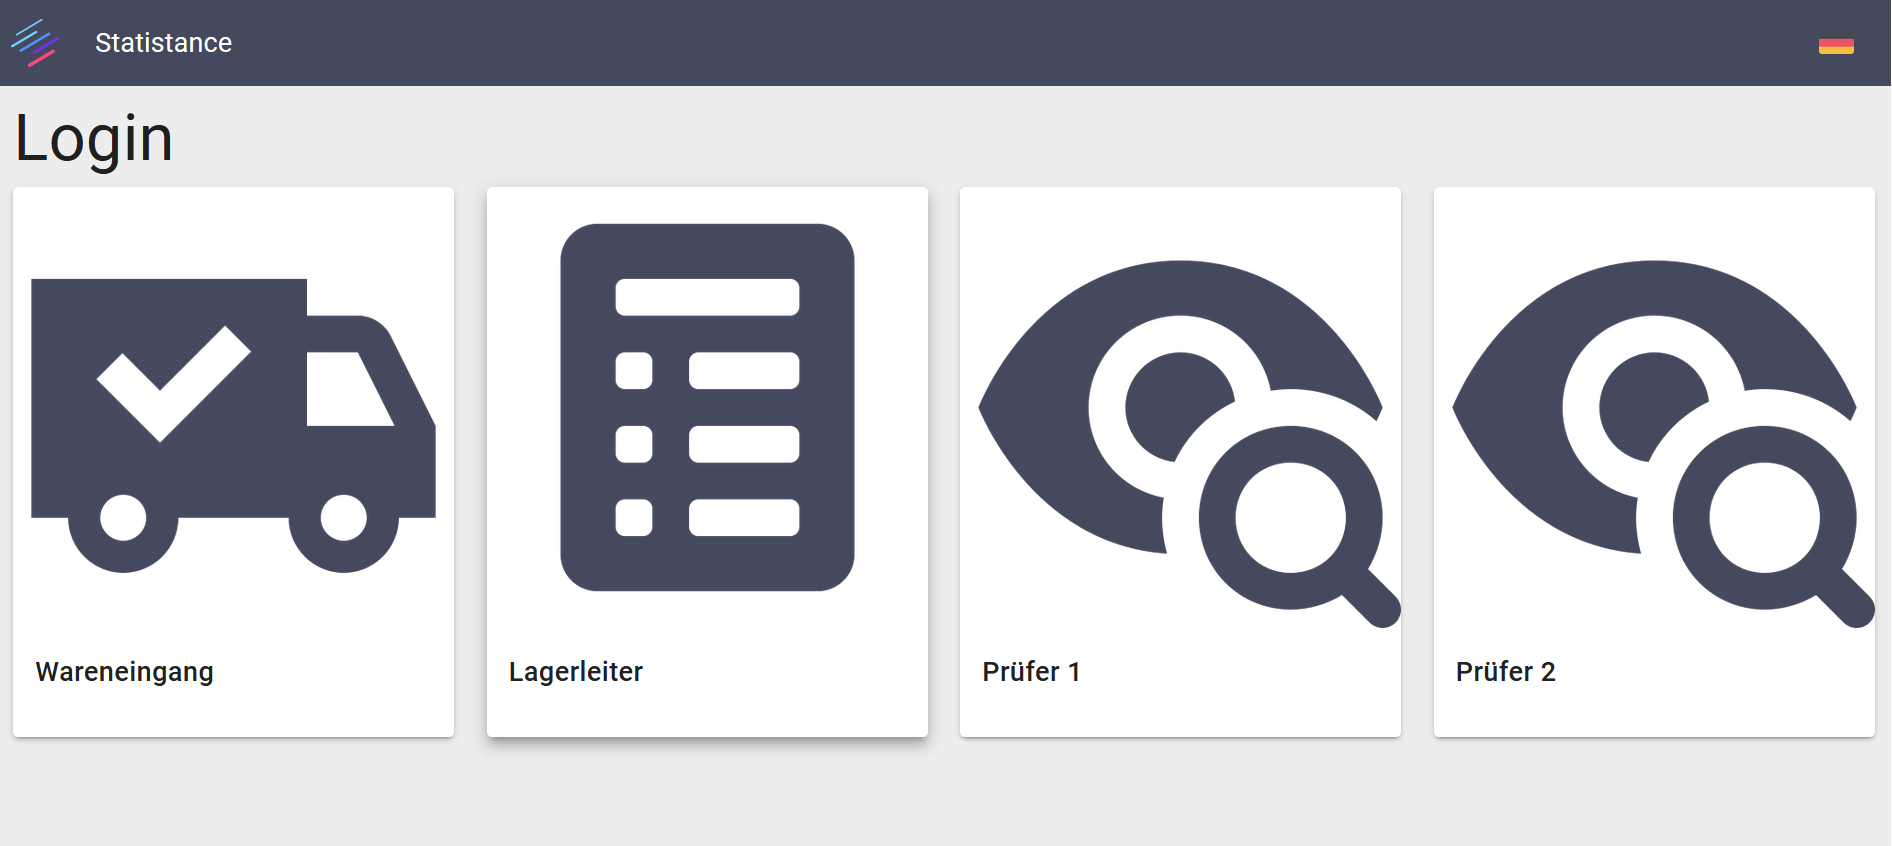
\includegraphics[width=15cm]{images/01_introduction/Statistance_StartPage.PNG}
\caption{Ansichten}
\label{fig:Startpage}
\end{figure}
Eine der Ansichten ist der Wareneingang. Dieser könnte wie in Abbildung \ref{fig:Wareneingang} aussehen. \cite{statistanceWareneingang} Abgeschlossene Lieferungen mit den entsprechenden Informationen, wie Produkte und Losumfang sowie zugewiesene Prüfer und der Fortschritt der Prüfung werden angezeigt. Auch Informationen zum Lieferanten, dem Lieferdatum sowie zum Mitarbeiter, welcher die Lieferung angenommen hat werden abgebildet.
\begin{figure}[!h]
\centering
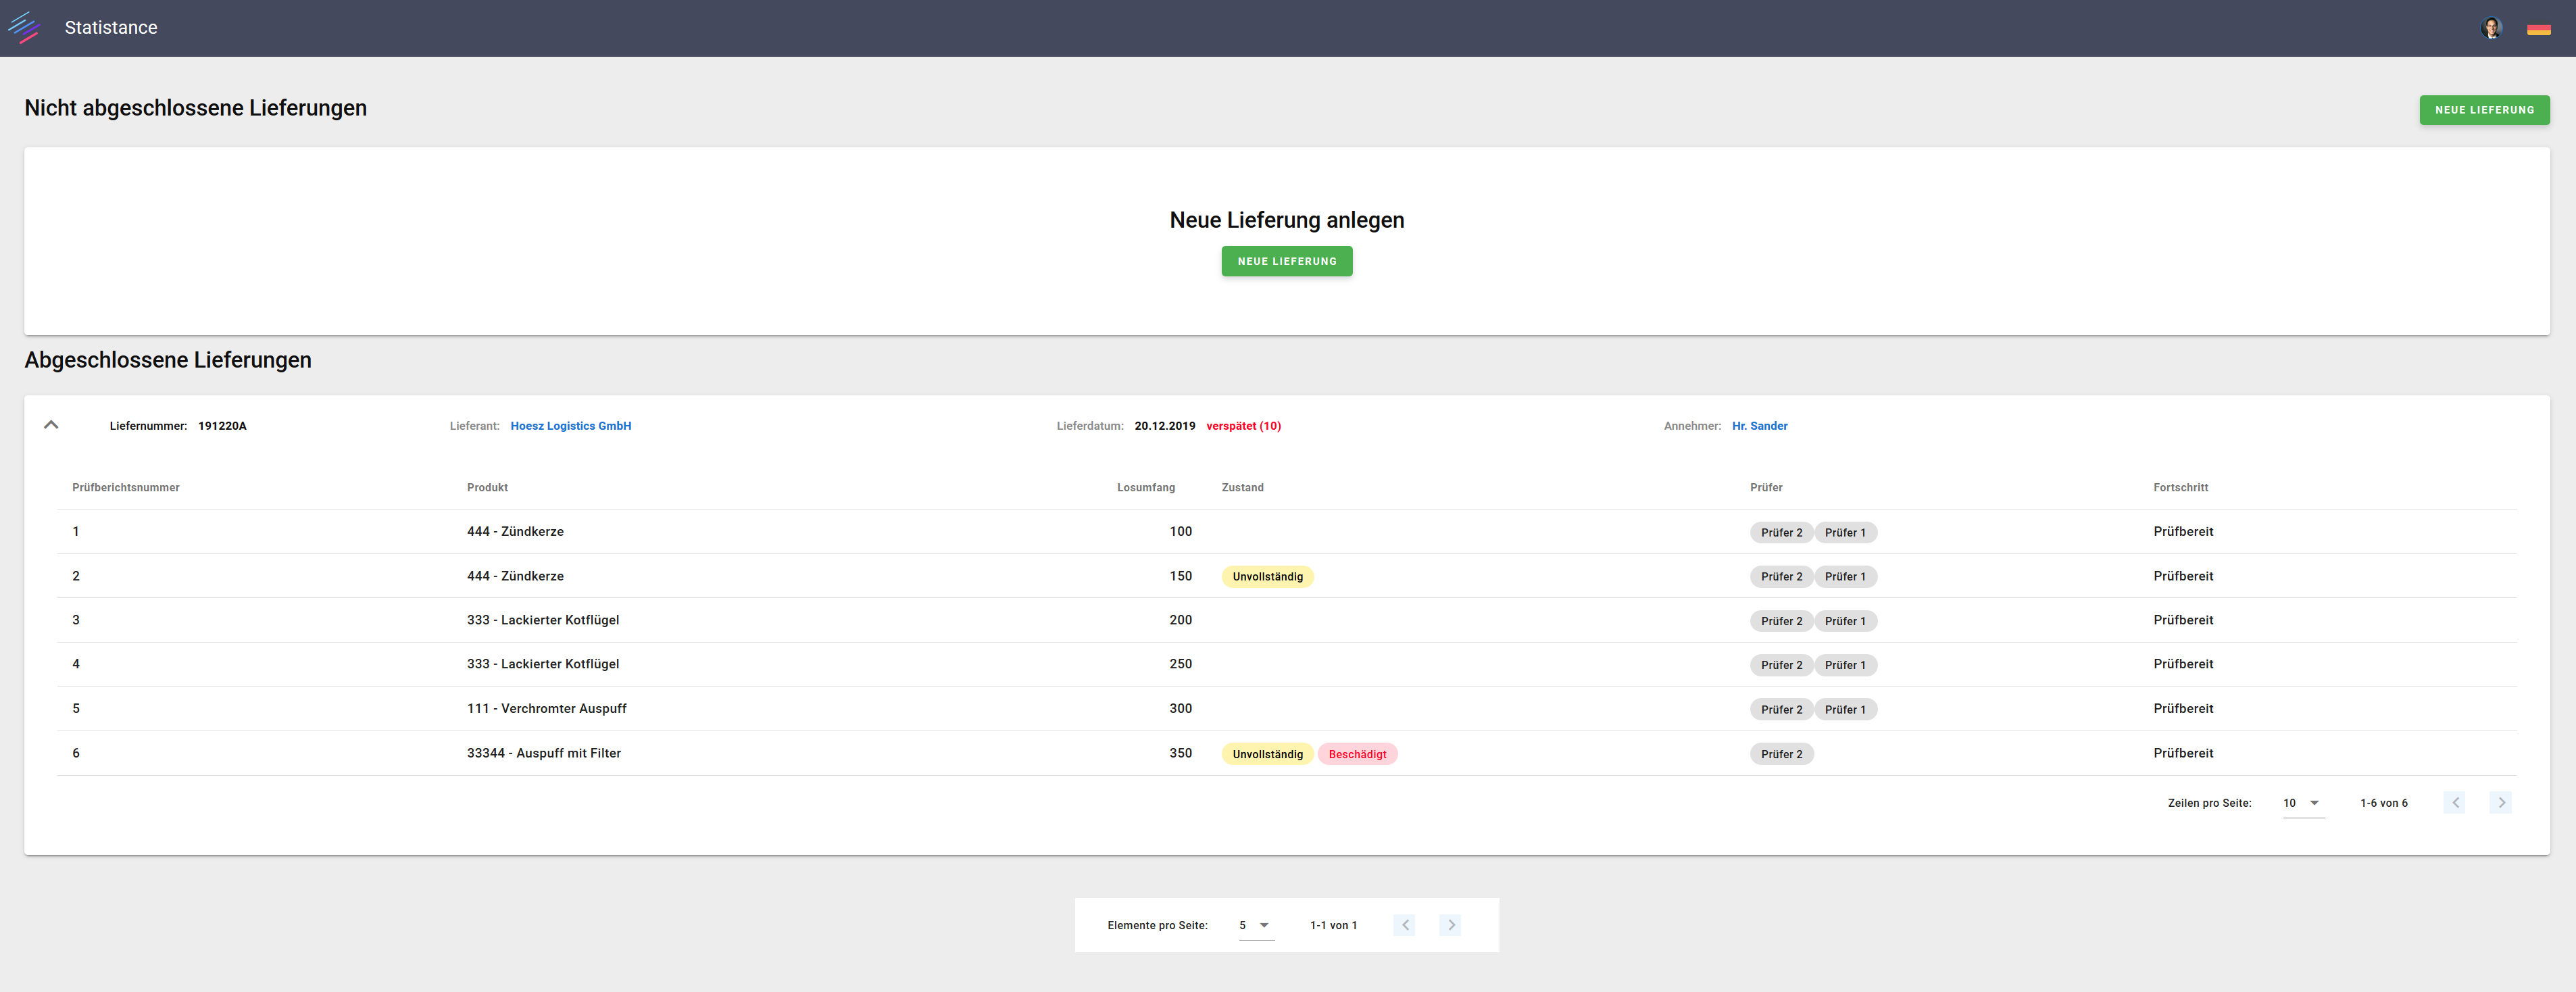
\includegraphics[width=15cm]{images/01_introduction/Statistance_Wareneingang.PNG}
\caption{Beispielhafte Ansicht des Wareneingangs eines Kunden}
\label{fig:Wareneingang}
\end{figure}


Statistance benötigt zur Bereitstellung des auf ERP-System-Daten basierenden Frontends und die statistischen Analysen, die Daten aus dem ERP-System des Kunden. Es werden Informationen zu Lieferanten, Bestellungen, Lieferungen, Produkten, Herstellern und Mitarbeitern für die weitere Verarbeitung benötigt.